\section{Đánh giá khả năng phát hiện bất thường}
\label{sec:danh_gia_bat_thuong}

Hệ thống học không giám sát nhằm nhận diện các mẫu dữ liệu chệch hướng so với phân phối chuẩn mà không cần gán nhãn trước \cite{ref_1_6}. Để xác thực năng lực này, đánh giá được tiến hành thông qua giả lập các kịch bản lỗi vật lý và phân tích sai số tái tạo trên mô hình TFLite thực tế.

\subsection{Thiết lập kịch bản kiểm thử với giả lập lỗi (Anomaly Injection)}

Hệ thống giả lập các lỗi vật lý trực tiếp trên đối tượng nghiên cứu để tạo ra các điểm bất thường có kiểm soát, tương tự các hư hỏng thường gặp:

\begin{itemize}
    \item \textbf{Mất cân bằng tải trọng (Load Imbalance):} Mô phỏng lệch lồng giặt bằng cách bố trí vật nặng dồn về một phía. Thử nghiệm này buộc hệ thống xử lý các biên độ gia tốc văng lớn bất thường, đặc biệt trong pha SPIN.
    \item \textbf{Biến động âm thanh:} Tạo tiếng ồn ma sát kim loại hoặc va đập nhân tạo để kiểm chứng độ nhạy của bộ lọc Mel 13 dải trước các dấu hiệu hỏng hóc vòng bi hoặc động cơ.
    \item \textbf{Trường hợp biên:} Áp dụng dịch chuyển biên độ và nhiễu biến thiên để kiểm chứng độ bền bỉ của mô hình trước các nhiễu nền ngẫu nhiên trong môi trường dân dụng.
\end{itemize}

\subsection{Phân tích phân phối sai số tái tạo}

Mô hình được kiểm chứng trên \textit{tập dữ liệu v6} — tập kiểm thử độc lập thu thập từ các phiên vận hành tách biệt hoàn toàn với dữ liệu huấn luyện, đảm bảo khả năng tổng quát hóa trước điều kiện môi trường thực tế. Phân tích biểu đồ MAE (Hình~\ref{fig:mae_sep_all}) cho thấy phân tách trạng thái rõ rệt:

\begin{itemize}
    \item \textbf{Pha GENTLE ($n=12.853$):} Mặc dù có cường độ tín hiệu thấp nhất và tập dữ liệu lớn nhất, mô hình duy trì sai số tái tạo bình thường ở mức cực thấp. Dữ liệu lỗi sau khi giả lập vượt hoàn toàn qua ngưỡng $\tau = 0{,}1241$, cho thấy độ nhạy của mô hình ngay cả ở trạng thái tĩnh.
    \item \textbf{Pha STRONG và SPIN:} Phân tách giữa hai cụm dữ liệu rõ nét. Đặc biệt ở pha SPIN, sai số MAE của dữ liệu bất thường tăng đáng kể so với ngưỡng $\tau = 0{,}0672$, cho phép hệ thống phát hiện lỗi văng lồng với độ tin cậy cao.
\end{itemize}

\begin{figure}[H]
    \centering
    \begin{subfigure}[b]{0.32\textwidth}
        \centering
        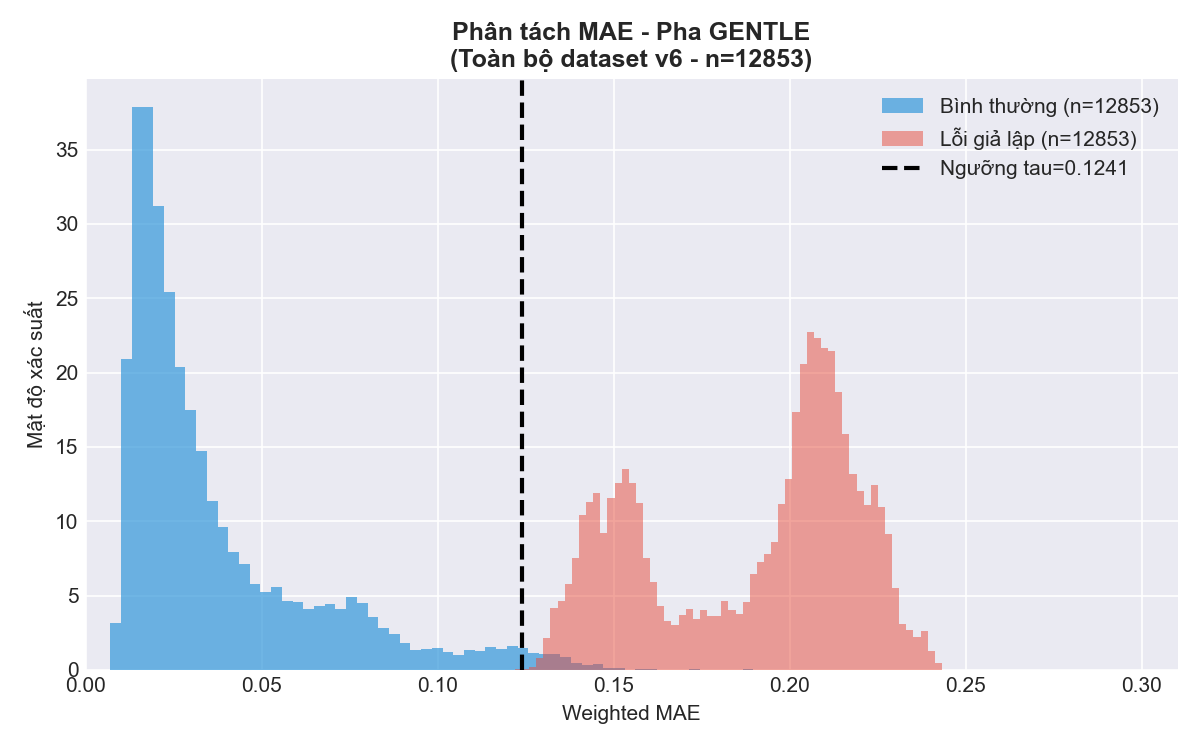
\includegraphics[width=\linewidth]{chap4/image/mae_sep_v11_GENTLE.png}
        \caption{Pha GENTLE ($n=12.853$)}
        \label{fig:mae_gentle}
    \end{subfigure}
    \hfill
    \begin{subfigure}[b]{0.32\textwidth}
        \centering
        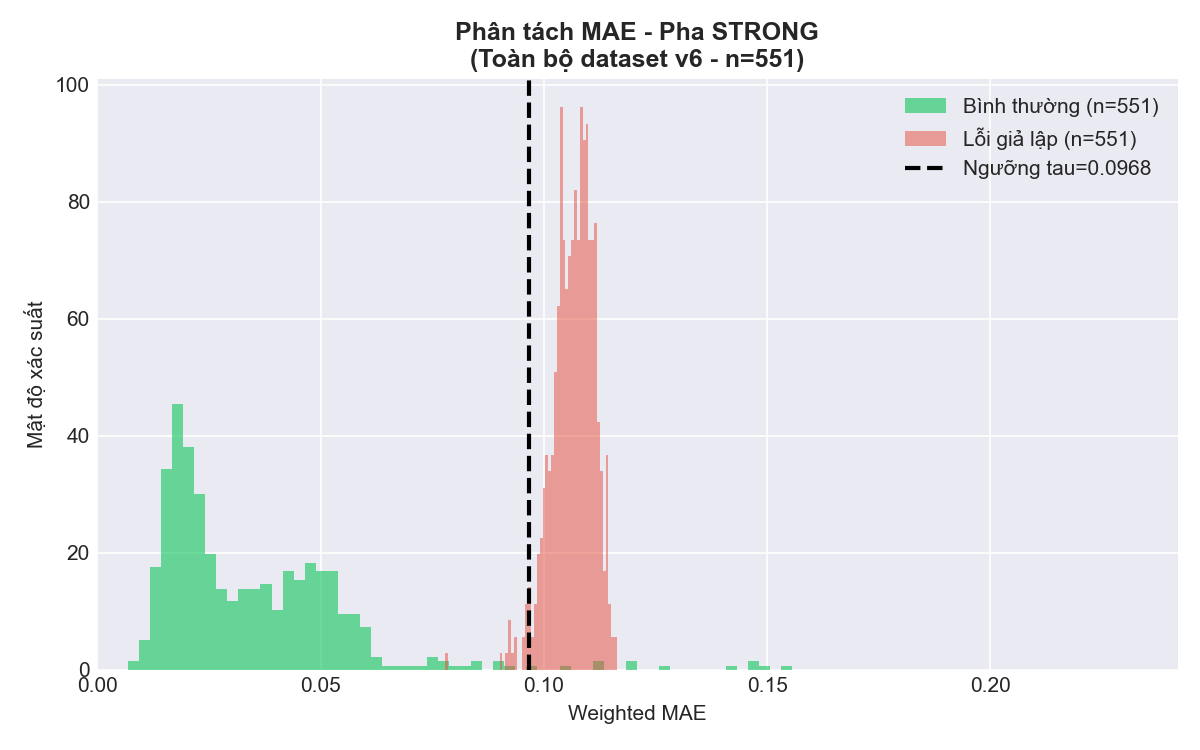
\includegraphics[width=\linewidth]{chap4/image/mae_sep_v11_STRONG.png}
        \caption{Pha STRONG ($n=551$)}
        \label{fig:mae_strong}
    \end{subfigure}
    \hfill
    \begin{subfigure}[b]{0.32\textwidth}
        \centering
        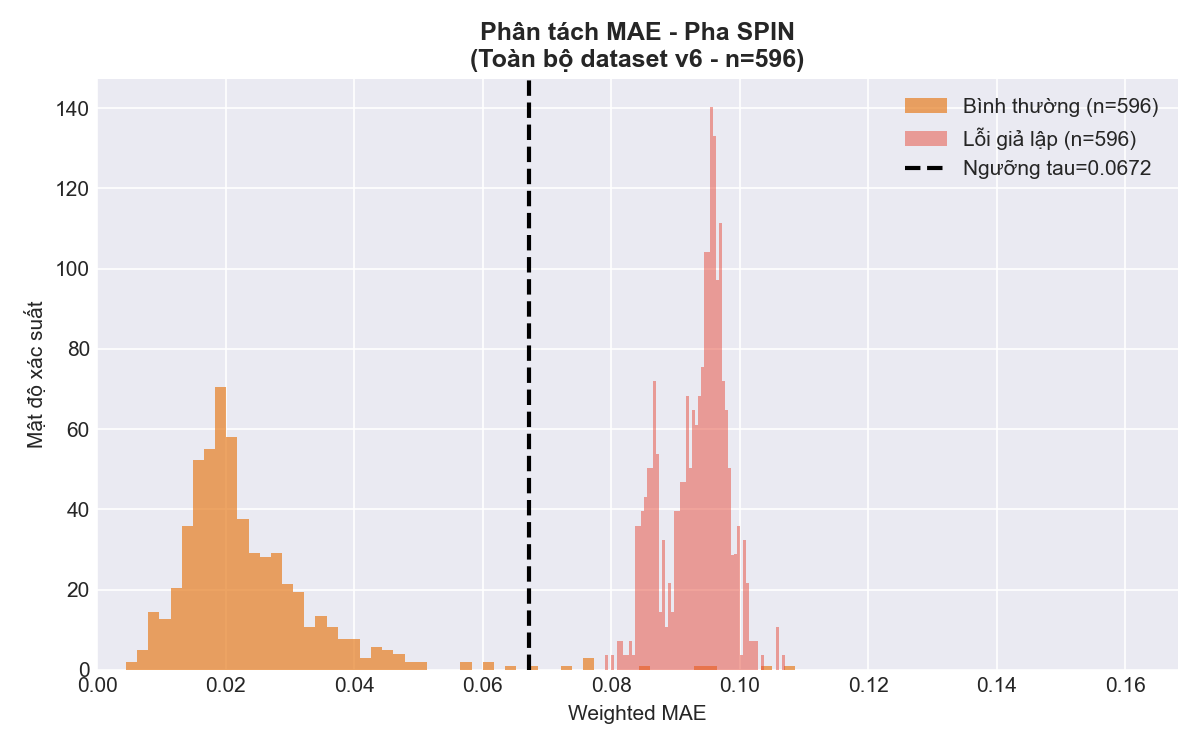
\includegraphics[width=\linewidth]{chap4/image/mae_sep_v11_SPIN.png}
        \caption{Pha SPIN ($n=596$)}
        \label{fig:mae_spin}
    \end{subfigure}
    \caption[Biểu đồ phân tách sai số MAE]{Biểu đồ phân tách sai số tái tạo MAE thực nghiệm trên mô hình v11. Mỗi pha vận hành được kiểm thử với tập dữ liệu tương ứng và tập lỗi giả lập ($n_{anomaly} \approx 500$ cho mỗi pha). Đường đứt nét biểu thị ngưỡng quyết định ($\tau$).}
    \label{fig:mae_sep_all}
\end{figure}

\subsection{Đánh giá độ nhạy và hiệu quả qua các chỉ số học máy}

Hiệu năng được đo lường qua chỉ số diện tích dưới đường cong ROC (AUC), F1-Score, Precision và Recall. Kết quả ghi nhận tại Bảng~\ref{tab:machine_learning_metrics}:

\begin{table}[H]
    \centering
    \caption[Chỉ số hiệu năng mô hình Ba trạng thái]{Chỉ số hiệu năng của mô hình tự mã hóa Ba trạng thái trên tập kiểm thử}
    \label{tab:machine_learning_metrics}
    \begin{tabular}{|l|c|c|c|c|}
    \hline
    \rowcolor[HTML]{EFEFEF}
    \textbf{Trạng thái} & \textbf{AUC} & \textbf{F1-Score} & \textbf{Precision} & \textbf{Recall} \\ \hline
    GENTLE & $0{,}9989$ & $0{,}9898$ & $0{,}9837$ & $0{,}9960$ \\ \hline
    STRONG & $0{,}9837$ & $0{,}9892$ & $0{,}9804$ & $0{,}9982$ \\ \hline
    SPIN   & $0{,}9993$ & $0{,}9967$ & $0{,}9933$ & $1{,}0000$ \\ \hline
    \end{tabular}
\end{table}

\subsection{Cơ chế lọc trễ thời gian và sự ổn định dài hạn}

Trong môi trường thực tế, sai số tức thời có thể vượt ngưỡng do nhiễu ngẫu nhiên. Vì vậy, firmware sử dụng cơ chế biểu quyết bất đối xứng đã trình bày tại Hình~\ref{fig:debounce_logic}: kích hoạt ALARM khi có ít nhất $5/10$ mẫu vượt ngưỡng và chỉ phục hồi về OK khi số mẫu vượt ngưỡng giảm xuống không quá $1/10$. Sự kết hợp giữa mô hình học sâu và bộ lọc thời gian giúp hệ thống phản ứng chính xác với các xung nhiễu, đảm bảo chỉ phát cảnh báo khi sự cố thực sự xảy ra.
